\documentclass[letterpaper,11pt]{article}

\usepackage{amsmath}
\usepackage{amssymb}
\usepackage{bm}
\usepackage[hmargin=1.25in,vmargin=1in]{geometry}
\usepackage{booktabs}
\usepackage{graphicx}
\usepackage{hyperref}
\usepackage{lmodern}
\usepackage{microtype}
\usepackage{pdflscape}
\usepackage{subcaption}

\title{Coursework 7: STAT 570}
\author{Philip Pham}
\date{\today}

\begin{document}
\maketitle
\begin{enumerate}
\item Create a binary variable $Z_i$, with $Z_i = 0$ corresponding to
  $Y_i \in \{0,1\}$ and $Z_i = 1$ corresponding to $Y_i \in \{2,3\}$. Let
  $q\left(x_i\right) = \mathbb{P}(Z_i = 1 \mid x_i)$, with
  $\mathbf{x}_i = \begin{pmatrix} 1 & x_{1i} & x_{2i}
  \end{pmatrix}^\intercal$, represent the probability of mental impairment being
  \emph{Moderate} or \emph{Impaired}, given covariates $\mathbf{x}_i$,
  $i = 1,\ldots,n = 40$.  Provide a single plot that shows the association
  between $q\left(x_i\right)$ and $x_{1i}$ and $x_{2i}$, on a response scale
  you feel is appropriate. Comment on the plot.

  \begin{figure}[h]
    \centering
    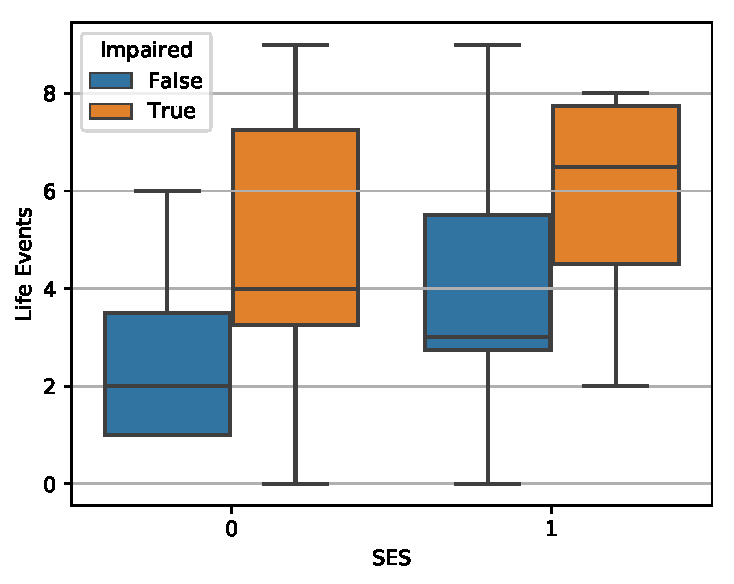
\includegraphics{p1_descriptive.pdf}
    \caption{Orange denotes $Z_i = 1$ and blue denotes $Z_i = 0$.}
    \label{fig:p1_descriptive}
  \end{figure}
  
  \begin{description}
  \item[Solution:] See Figure \ref{fig:p1_descriptive}. Conditioned on SES,
    those that are impaired ($Z_i = 1$) have a greater number of life events on
    average.
  \end{description}
\item Suppose $Z_i \mid q_i \sim \operatorname{Binomial}\left(1, q_i\right)$
  independently for $i = 1,\ldots, n = 40$, where $q_i =
  q\left(x_i\right)$. Consider the logistic regression model,
  \begin{equation}
    q\left(x_i\right) = \log\left(
      \frac{q\left(\mathbf{x}_i\right)}{1 - q\left(\mathbf{x}_i\right)}
    \right)
    =
    \mathbf{x}_i^\intercal \bm{\gamma}
    = \gamma_0 + \gamma_1 x_{1i} + \gamma_2 x_{2i},
    \label{eqn:p2_model}
  \end{equation}  
  where $\bm{\gamma} = \begin{pmatrix}\gamma_0 & \gamma_1 & \gamma_2
  \end{pmatrix}^\intercal$. Write down the log-likelihood
  $l\left(\bm{\gamma}\right)$ for the sample $z_i$, $i = 1,\ldots, n$.

  \begin{description}
  \item[Solution:] Solving for $q\left(\mathbf{x}_i\right)$ in Equation
    \ref{eqn:p2_model}, we find
    \begin{equation}
      q\left(\mathbf{x}_i\right)
      = \frac{\exp\left(\mathbf{x}_i^\intercal \bm{\gamma}\right)}
      {1 + \exp\left(\mathbf{x}_i^\intercal \bm{\gamma}\right)}
      = \frac{1}
      {1 + \exp\left(-\mathbf{x}_i^\intercal \bm{\gamma}\right)}.
      \label{eqn:p2_qi}
    \end{equation}

    The likelihood function is
    $L\left( \bm{\gamma} \right) = \prod_{i=1}^n
    \left(q\left(\mathbf{x}_i\right)\right)^{z_i} \left(1 -
      q\left(\mathbf{x}_i\right)\right)^{1 - z_i}$, so the log-likelihood
    function becomes
    \begin{align}
      l\left(\bm{\gamma}\right)
      &= \log L\left( \bm{\gamma} \right)
        = \sum_{i=1}^n \left(
        z_i \log q\left(\mathbf{x}_i\right)
        +
        \left(1 - z_i \right) \log\left(1 - q\left(\mathbf{x}_i\right)\right)
        \right)
        \label{eqn:p2_log_likelihood}\\
      &= \sum_{i=1}^n\left(
        z_i\log\frac{q\left(\mathbf{x}_i\right)}{1 -q\left(\mathbf{x}_i\right)}
        + \log\left(1 -q\left(\mathbf{x}_i\right)\right)
        \right) \nonumber\\
      &= \sum_{i=1}^n
        \left(
        z_i\mathbf{x}_i^\intercal\bm{\gamma} +
        \log\frac{1}{1 + \exp\left(\mathbf{x}_i^\intercal\bm{\gamma}\right)}
        \right)
        = \sum_{i=1}^n
        -\log\left(
        1 + \exp\left(\left(1 - 2z_i\right)\mathbf{x}_i^\intercal\bm{\gamma}\right)
        \right). \nonumber
    \end{align}
  \end{description}
\item Fit the model described in the previous part, and give confidence
  intervals for the odds ratios.

  Carefully interpret these odds ratios.

  \begin{table}[!h]
    \centering
    \begin{tabular}{lrrrr}
\toprule
{} &  Estimate &  Standard error &  95\% CI lower bound &  95\% CI upper bound \\
\midrule
$\gamma_0$ & -0.925065 &        0.723346 &            -2.342797 &             0.492666 \\
$\gamma_1$ & -1.629731 &        0.780849 &            -3.160167 &            -0.099296 \\
$\gamma_2$ &  0.309899 &        0.147920 &             0.019980 &             0.599818 \\
\bottomrule
\end{tabular}

    \caption{Estimates and confidence intervals for $\hat{\bm\gamma}$ using
      maximum likelihood estimation.}
    \label{tab:p3_gamma_hat}
  \end{table}
  
  \begin{description}
  \item[Solution:] Taking the derivative of Equation
    \ref{eqn:p2_log_likelihood}, we have the score function:

    \begin{align}
      S\left(\bm\gamma\right)
      = \nabla^\intercal l\left(\bm\gamma\right)
      &= \sum_{i=1}^n \frac{2z_i - 1}{1 + \exp\left(
        \left(1 - 2z_i\right)\mathbf{x}_i^\intercal\bm{\gamma}
        \right)}\exp\left(
        \left(1 - 2z_i\right)\mathbf{x}_i^\intercal\bm{\gamma}
        \right)\mathbf{x}_i.
        \nonumber\\
      &= \sum_{i=1}^n \frac{2z_i - 1}{1 + \exp\left(
        \left(2z_i - 1\right)\mathbf{x}_i^\intercal\bm{\gamma}
        \right)}\mathbf{x}_i \nonumber\\
      &= X^\intercal\left(
        \mathbf{z} - \mathbf{q}\left(X\right)
        \right),
    \label{eqn:p3_score_function}
    \end{align}
    where
    $\mathbf{z} = \begin{pmatrix}z_1 & z_2 & \cdots & z_n\end{pmatrix}^\intercal$ and
    $\mathbf{q}\left(X\right) = \begin{pmatrix}q_1 & q_2 &
      \cdots & q_n\end{pmatrix}^\intercal$.
    
    From Equation \ref{eqn:p3_score_function}, we have the Fisher information
    matrix:
    \begin{align}
      I_n\left(\bm\gamma\right)
      &= \operatorname{var}\left(S\left(\bm\gamma\right) \mid \bm\gamma\right)
        = \mathbb{E}\left[
        S\left(\bm\gamma\right)
        S\left(\bm\gamma\right)^\intercal
        \mid \bm\gamma
        \right] \nonumber\\
      &= \mathbb{E}\left[
        X^\intercal\left(
        \mathbf{z} - \mathbf{q}\left(X\right)
        \right)
        \left(
        \mathbf{z} - \mathbf{q}\left(X\right)
        \right)^\intercal
        X \mid \bm\gamma
        \right] \nonumber \\
      &= X^\intercal\mathbb{E}\left[
        \left(
        \mathbf{z} - \mathbf{q}\left(X\right)
        \right)
        \left(
        \mathbf{z} - \mathbf{q}\left(X\right)
        \right)^\intercal
        \mid \bm\gamma
        \right]X \nonumber\\
      &= \sum_{i=1}^n 
        q\left(\mathbf{x}_i\right)
        \left(1 - q\left(\mathbf{x}_i\right)\right)
        \mathbf{x}_i\mathbf{x}_i^\intercal
        =
        \sum_{i=1}^n
        \frac{1}{2 + \exp\left(
        -\mathbf{x}_i^\intercal \bm\gamma
        \right) + \exp\left(
        \mathbf{x}_i^\intercal \bm\gamma
        \right)}
        \mathbf{x}_i\mathbf{x}_i^\intercal
        ,
        \label{eqn:p3_fisher_information}
    \end{align}
    where we have used independence of the observations and variance of the
    binomial distribution to get the last line.

    We solve Equation \ref{eqn:p3_score_function},
    $S\left(\hat{\bm{\gamma}}\right) = \mathbf{0}$, to get an estimate for
    $\bm\gamma$. Using Equation \ref{eqn:p3_fisher_information}, we have that
    \begin{equation}
      \hat{\bm\gamma}
      \xrightarrow{\mathcal{D}}
      \mathcal{N}\left(
        \gamma,
        I_n^{-1}\left(\hat{\bm\gamma}\right)
      \right),
      \label{eqn:p3_gamma_hat_dist}
    \end{equation}
    that is, $\hat{\bm\gamma}$ is asymptotically normal.

    Using Equation \ref{eqn:p3_gamma_hat_dist}, we obtain the estimates and
    intervals in Table \ref{tab:p3_gamma_hat}.

    The predicted log odds ratio given some $\mathbf{x}_i$ is
    \begin{equation}
      \hat\theta_i = \mathbf{x}_i^\intercal\hat{\bm\gamma},
      \label{eqn:p3_prediction}
    \end{equation}
    which will have variance
    \begin{equation}
      \operatorname{var}\left(\hat\theta_i\right)
      = \mathbf{x}_i^\intercal\operatorname{var}\left(\hat{\bm\gamma}\right)
      \mathbf{x}_i
      \approx \mathbf{x}_i^\intercal I_n^{-1}\left(\hat{\bm\gamma}\right)
      \mathbf{x}_i,
      \label{eqn:p3_prediction_variance}
    \end{equation}
    using Equation \ref{eqn:p3_gamma_hat_dist}.
  \end{description}
\end{enumerate}
\end{document}
